O algoritmo \algname{Parallel U-Curve Search (PUCS)} foi desenvolvido 
para resolver o problema U-Curve particionando o espaço de busca em 
partes que podem ser resolvidas independentemente e de forma paralela. 
Além disso, a dinâmica desse algoritmo depende de parâmetros que 
determinam o tempo de execução e qualidade da solução obtida, permitindo
ao usuário adequar o algoritmo aos recursos computacionais disponíveis. 

\section{Princípios}\label{sec:pucs_principles}
Seja $S$ o conjunto de características do problema em questão. O 
primeiro passo do particionamento é escolher arbitrariamente $S'$ um 
subconjunto de $S$; de maneira complementar, definimos 
$\overline{S'} = S \setminus S'$. Agora, sejam $X, Y \in \powerset (S)$
e $\sim$ a relação:

\begin{equation*}
    X \sim Y \iff (X \cap S') = (Y \cap S')
\end{equation*}
Esta relação é de equivalência, pois nela valem:

\begin{itemize}
    \item{reflexividade}
        \begin{align*} 
            X \sim X \text{, pois }
            (X \cap S') = (X \cap S')
        \end{align*} 
    \item{simetria}
        \begin{align*}
            X \sim Y  & \iff \\
            (X \cap S') = (Y \cap S') & \iff \\
            (Y \cap S') = (X \cap S') & \iff \\
            Y \sim X 
        \end{align*}
    \item{transitividade,}
        \begin{align*}
            X \sim Y, Y \sim Z & \Rightarrow \\
            (X \cap S') = (Y \cap S') = (Z \cap S') & \Rightarrow \\
            (X \cap S') = (Z \cap S') & \Rightarrow \\
            X \sim Z
        \end{align*}
\end{itemize}
Portanto, o conjunto das classes de equivalência definidas por $\sim$ é
uma partição do espaço de busca original. Tome como exemplo o conjunto
$S = \{a, b, c\}$; se $S' = {a}$, então existem duas classes de 
equivalência no particionamento do espaço de busca que definimos, 
formados pelos conjuntos $\{\emptyset, b, c, bc\}$ e $\{a, ab, ac, 
abc\}$.

Pela definição da relação $\sim$ temos que a presença de cada 
característica de $S'$ em uma dada parte do reticulado não muda, isto é,
ou ela está presente em todos subconjuntos da parte ou não está presente
em nenhum, portanto, dizemos que estas variáveis são {\bf fixas}. De 
modo análogo, as variáveis de $\overline{S'}$ são {\bf livres}. Tanto 
variáveis fixas quanto livres podem definir reticulados Booleanos junto 
a relação de ordem parcial $\subseteq$.

O conjunto $\powerset (S')$ induz um reticulado Booleano em que cada
elemento representa uma classe de equivalência do espaço de soluções
do problema original, chamamos este de {\bf reticulado externo}. Para 
cada classe de equivalência (nó do reticulado externo), o conjunto 
$\powerset (\overline {S'})$ induz um outro reticulado Booleano ({\bf
reticulado interno}) em que cada elemento representa um subconjunto de
problema original. Seja $A \in \powerset (S')$ um elemento do reticulado 
externo, então cada $B \in \powerset (\overline{S'})$ do reticulado 
interno em $A$ representa o conjunto $X = B \cup A$ do espaço de busca
do problema original. A figura ~\ref{fig:pucs_parts} apresenta um 
exemplo de particionamento feito pelo \algname{PUCS} em um reticulado 
Booleano com cinco características.

\begin{figure}[!ht]
  \centering 
  \begin{tabular}{c c}
    \subfigure[] {\scalebox{0.4}{
     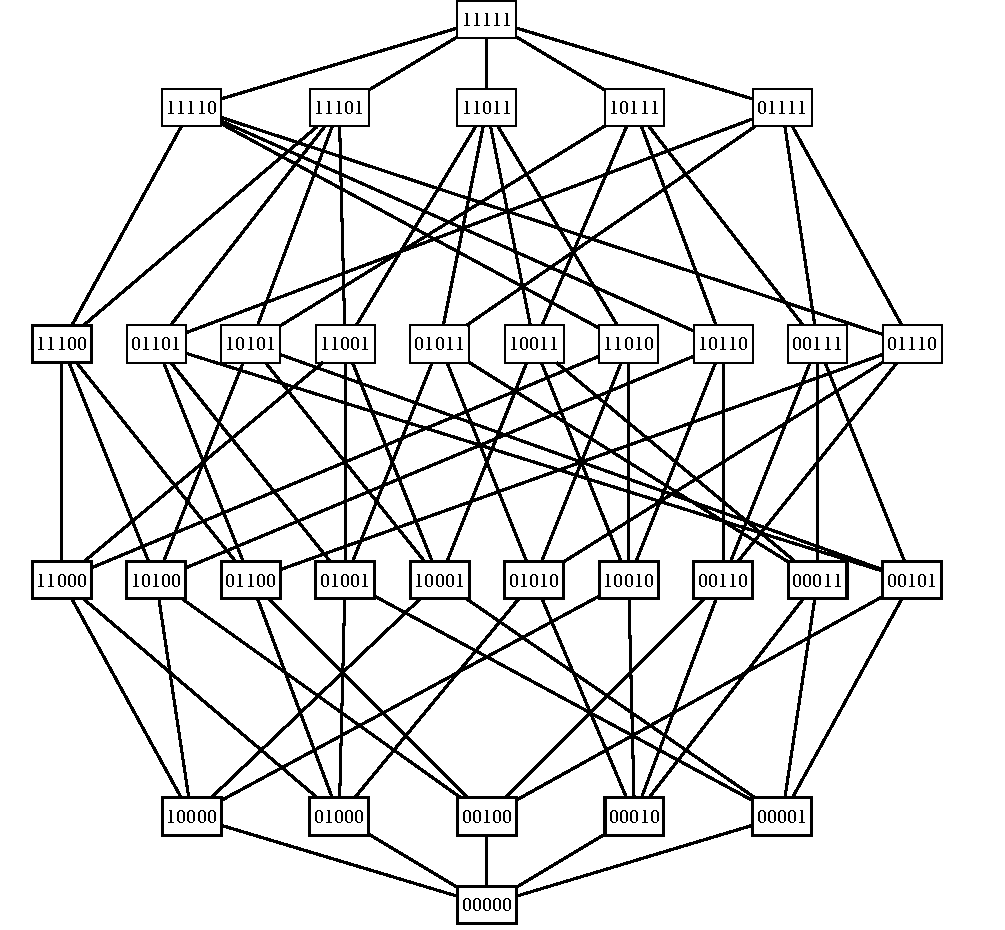
\includegraphics[clip=true]{pucs/partition/full_lattice.pdf}}
     \label{fig:pucs_part:full} }
    & 
    \subfigure[] {\scalebox{1}{
    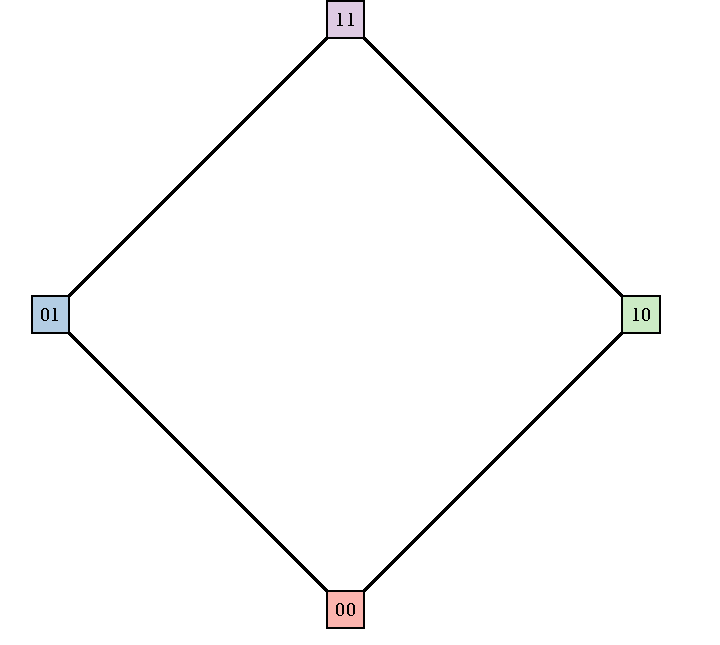
\includegraphics[clip=true]{pucs/partition/external_lattice.pdf}}
    \label{fig:pucs_part:external} }
    \\
    \subfigure[] {\scalebox{1}{
    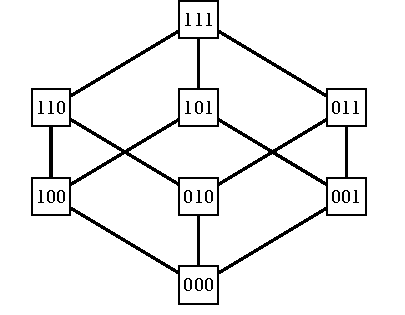
\includegraphics[clip=true]{pucs/partition/internal_lattice.pdf}}
    \label{fig:pucs_part:internal} }
    &
    \subfigure[] {\scalebox{0.4}{
    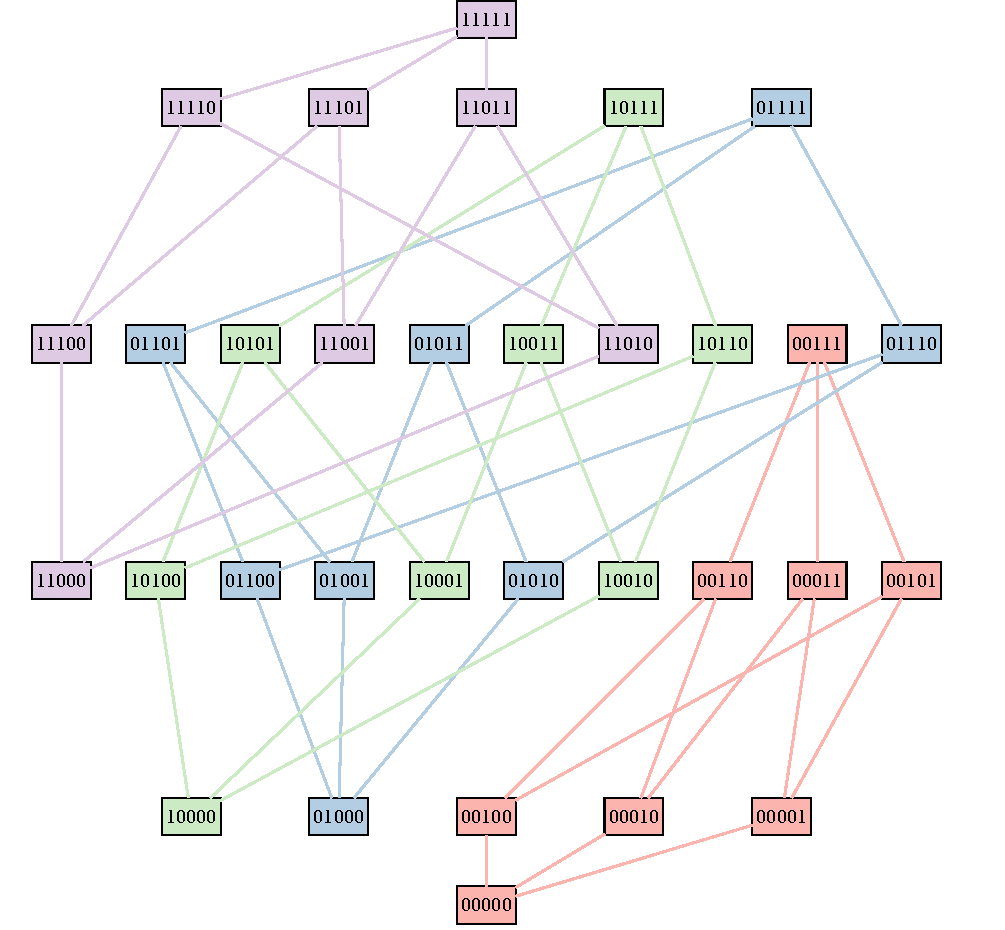
\includegraphics[clip=true]{pucs/partition/all_parts.pdf}}
    \label{fig:pucs_part:parts} }   
    \\
  \end{tabular}
    \caption{Exemplo de particionamento feito pelo algoritmo 
    \algname{PUCS} em uma instância com cinco características; o 
    reticulado Booleano desta instância é representado na figura 
    ~\ref{fig:pucs_part:full}. Neste particionamento, as duas primeiras
    variáveis formam o conjunto de variáveis fixadas, definindo o 
    reticulado externo (figura ~\ref{fig:pucs_part:external}) enquanto 
    as outras três definem os reticulados internos, que são cópias do
    reticulado da figura ~\ref{fig:pucs_part:internal}. A figura 
    ~\ref{fig:pucs_part:parts} mostra o reticulado Booleano original, sem
    as arestas que ligam duas partes diferentes, e a cor de cada nó 
    representa a qual parte tal nó pertence, de acordo com as cores
    do reticulado externo em ~\ref{fig:pucs_part:external}
    Note que, de fato, 
    cada parte forma um reticulado pequeno de mesmo tamanho e com mesma 
    estrutura que o reticulado da figura ~\ref{fig:pucs_part:internal}}
  \label{fig:pucs_parts} 
\end{figure}

Os reticulados internos e externo elucidam a estrutura recursiva do 
problema de seleção de características e sugerem que podemos construir 
uma solução ao problema original a partir de soluções de outros 
problemas, sobre os reticulados externo e internos, abordagem conhecida
em computação como divisão e conquista. Seja $\langle S, c \rangle$ uma 
instância do problema de seleção de características, $S'$ o conjunto de 
variáveis fixas, $\overline{S'}$ o conjunto de variáveis livres, e 
$A \in \powerset (S')$ um subconjunto que é nó do reticulado externo, 
então podemos definir um outro problema de seleção de características 
$\langle \overline{S'}, c_{A} \rangle$ em que 
\begin{align*}
    c_{A} (X) = c (X \cup A).
\end{align*}
Resolver a instância $\langle \overline{S'}, c_{A} \rangle$ é 
essencialmente achar o mínimo do problema inicial restrito a classe de
equivalência de $A$, dizemos também que estamos resolvendo a parte $A$. 
Se soubermos em qual classe o mínimo global reside, podemos resolver 
apenas tal parte e garantir que a solução encontrada é a solução do 
problema original.


\section{Dinâmica}
Com as estruturas de reticulado interno e externo, o \algname{PUCS} 
resolve uma instância do problema U-Curve em duas etapas. Na primeira, o
algoritmo percorre o reticulado externo, fazendo podas sempre que 
possível, e armazena cada parte que é candidata a conter o mínimo global
do problema. Na segunda etapa, para cada parte candidata, resolve-se o
problema U-Curve auxiliar que é equivalente ao problema original, mas 
restrito a parte de interesse; em seguida, escolhe-se como resposta o 
conjunto custo mínimo entre as soluções dos problemas parciais.


\subsection{Condições de poda}
As podas eliminam do reticulado externo intervalos da forma 
$[X, \powerset(S')]$ ou $[\emptyset, X]$ e são realizadas sempre que a 
hipótese de curva em U implica que todas as partes contidas nestes 
intervalos não contém o mínimo global. Para entender o critério de poda,
vamos definir que a {\bf ponta superior} de um reticulado Booleano 
$\powerset (A)$ é o próprio conjunto $A$ e a {\bf ponta inferior} deste
reticulado é o conjunto vazio. Note que no reticulado interno de uma
parte $P$ a ponta inferior representa o próprio conjunto de 
características $P$, enquanto que a ponta superior representa o conjunto
de características $P \cup \overline{S'}$.

\begin{mytheorem}[Critério de poda para o reticulado externo do 
algoritmo \algname{PUCS}]
\label{theorem:pucs:pruning}
Sejam $S$ um conjunto de características e $S'$ um conjunto de variáveis
fixas no particionamento definido pelo algoritmo \algname{PUCS}. Dados
$P, Q \in \powerset (S')$ dois elementos do reticulado externo com 
$Q \subseteq P$; se a ponta inferior do reticulado interno de $P$ tem 
custo maior do que a ponta inferior do reticulado interno de $Q$, então 
todas as partes do intervalo $[P, \powerset (S')]$ tem apenas conjuntos 
de características com custo maior do que o custo da ponta inferior de 
$Q$.
\end{mytheorem}
\begin{proof}
Se o custo da ponta inferior do reticulado interno de $P$ é maior do que
a de $Q$, então:

\begin{align*}
    c_Q (\emptyset) & < c_P (\emptyset) \\
    c (\emptyset \cup Q) & < c (\emptyset \cup P) \\
    c (Q) & < c (P) 
\end{align*}

Como $Q \subseteq P$, temos que existe uma cadeia que passa pelas pontas
inferiores de $Q$ e $P$. Além disso, para qualquer conjunto de 
características $X \in \powerset (S)$, com $P \subseteq X$, a hipótese 
de curva em U garante que:
\begin{align*}
    c (P) & \leq max \{c (Q), c (X)\}
\end{align*}
e como $c (P) > c (Q)$, temos que $c (X) \geq c (P)$, isto é, qualquer 
elemento do reticulado Booleano original que cobre a ponta inferior de 
$P$ tem custo estritamente maior do que o custo da ponta inferior de $Q$.
Note que para qualquer parte $R$ do intervalo $[P, \powerset (S')]$, 
vale que $P \subseteq R$, e como a ponta inferior de $P$ não contém 
nenhum elemento de $\overline {S'}$, então qualquer conjunto de 
características da parte $R$ cobre a ponta inferior de $P$ e portanto 
tem custo estritamente maior do que o custo da ponta inferior da parte 
$Q$.
\end{proof}

\begin{mytheorem}[Critério dual de poda para o reticulado externo do 
algoritmo \algname{PUCS}]
\label{theorem:pucs:pruning_dual}
Sejam $S$ um conjunto de características e $S'$ um conjunto de variáveis
fixas no particionamento definido pelo algoritmo \algname{PUCS}. Dados
$P, Q \in \powerset (S')$ dois elementos do reticulado externo com 
$Q \subseteq P$; se a ponta superior do reticulado interno de $P$ tem 
custo menor do que a ponta superior do reticulado interno de $Q$, então 
todas as partes do intervalo $[\emptyset, Q]$ tem apenas conjuntos 
de características com custo maior do que o custo da ponta superior de 
$P$.
\end{mytheorem}

\begin{proof}
Se o custo da ponta superior do reticulado interno de $Q$ é maior do que
a de $P$, então:

\begin{align*}
    c_P (\overline{S'}) & < c_Q (\overline{S'}) \\
    c (\overline{S'} \cup P) & < c (\overline{S'} \cup Q) \\
\end{align*}

Como $Q \subseteq P$, temos que existe uma cadeia que passa pelas pontas
superiores de $Q$ e $P$. Além disso, para qualquer conjunto de 
características $X \in \powerset (S)$, com $\{Q \cup \overline{S'}\}\supseteq X$, a hipótese 
de curva em U garante que:
\begin{align*}
    c (Q \cup \overline{S'}) \leq max \{c (P \cup \overline{S'}), c (X)\}
\end{align*}
e como $c (Q \cup \overline{S'}) > c (P \cup \overline{S'})$, temos que 
$c (X) \geq c (Q \cup \overline{S'})$, isto é, qualquer elemento do reticulado Booleano 
original que é coberto pela ponta superior de $Q$ tem custo estritamente maior 
do que o custo da ponta superior de $P$. Note que para qualquer parte 
$R$ do intervalo $[\emptyset, Q]$, vale que $R \subseteq Q$, e como 
a ponta superior de $Q$ contém todos os elementos de $\overline {S'}$, 
então qualquer conjunto de características da parte $R$ é coberto pela 
ponta superior de $Q$ e portanto tem custo estritamente maior do que o 
custo da ponta superior da parte $P$.
\end{proof}

\subsection{Passeio aleatório no reticulado externo}
O passeio do \algname{PUCS} se inicia escolhendo arbitrariamente um nó 
inicial que pertence ao espaço de busca, então a cada passo escolhe-se 
aleatoriamente um vizinho do nó corrente, que também deve pertencer ao 
espaço de busca, e verificam-se as condições de poda. Caso elas sejam 
verdadeiras, o procedimento de poda elimina parte do reticulado; se o 
vizinho escolhido foi removido nesta etapa, então escolhe-se outro 
vizinho. O vizinho escolhido torna-se então o nó corrente e o 
procedimento é repetido até que não seja possível escolher um vizinho; 
quando isto ocorre e o espaço ainda não foi esgotado, escolhe-se 
novamente um início de passeio arbitrariamente. Todo nó visitado é 
automaticamente removido do espaço de busca, e os passeios aleatórios
são repetidos até que o espaço de busca tenha sido esgotado, ou seja,
todo nó foi ou visitado ou removido em alguma poda.

Durante a realização dos passeios aleatórios, precisamos armazenar quais
são as partes candidatas a conterem o mínimo global. As podas deste 
algoritmo removem do espaço de busca apenas partes que obrigatoriamente 
não contém o mínimo global, portanto qualquer outra parte é candidata a 
conter tal elemento. Desta forma, como toda parte é visitada ou podada, 
temos que o conjunto de nós visitados e não podados é exatamente o 
conjunto de candidatos a conterem o subconjunto de custo ótimo.

% TODO: acho que isso tem mais a ver com a implementação
%Sempre que um nó do reticulado externo é podado ou visitado ele deve ser
%removido do espaço de busca, e representar este espaço explicitamente 
%não é uma boa solução devido ao seu tamanho, que é exponencial em 
%relação a quantidade de características fixas. A estrutura de dados 
%utilizada deve ser eficiente tanto para inserções (de intervalos e de 
%pontos do reticulado) quanto para consultas. Escolhemos para este 
%algoritmo 

As figuras ~\ref{fig:pucs:example:part_1} - 
~\ref{fig:pucs:example:part_3} mostram a dinâmica do \algname{PUCS} ao
resolver uma instância do problema U-Curve.

\begin{figure}[!ht]
    \begin{center}
    \begin{tabular}{l r}
    \centering
        \subfigure[] {
        \label{fig:pucs:example:lattice}
        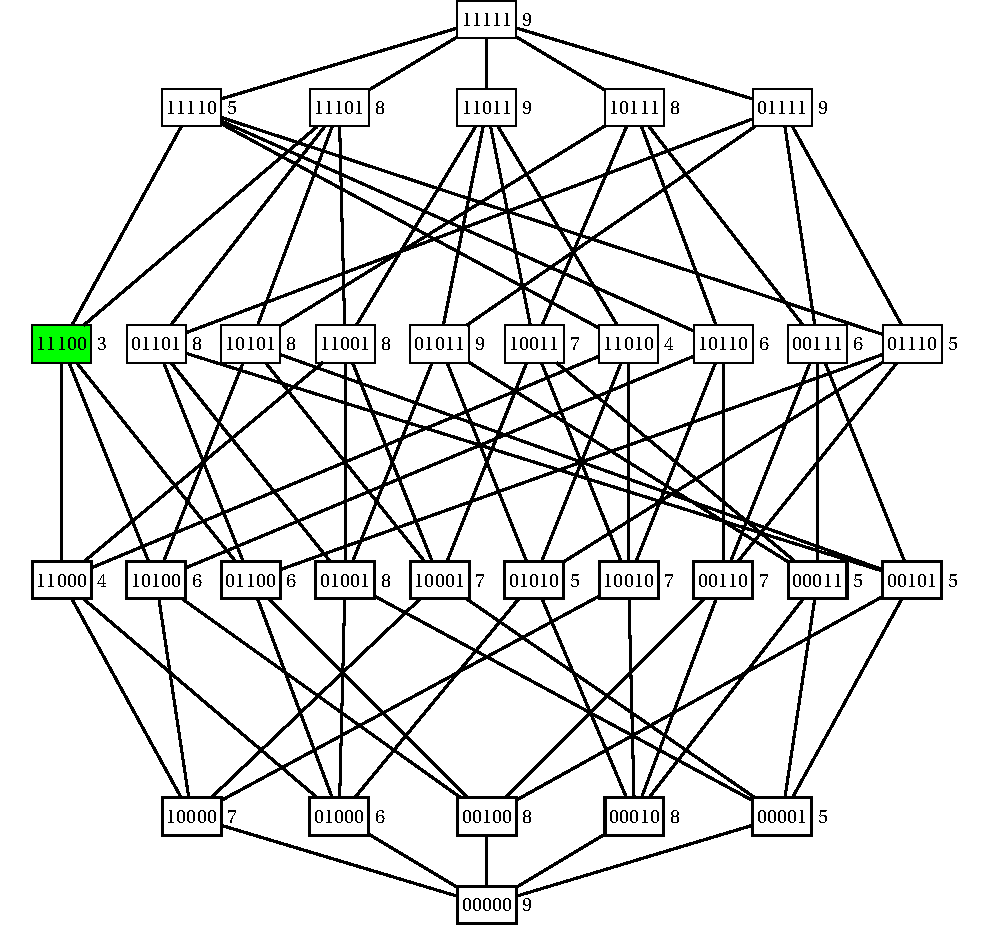
\includegraphics[clip=true, width=0.48\textwidth]{pucs/sample_run/Boolean_lattice.pdf}
    }
    &
        \subfigure[] {
        \label{fig:pucs:example:A}
        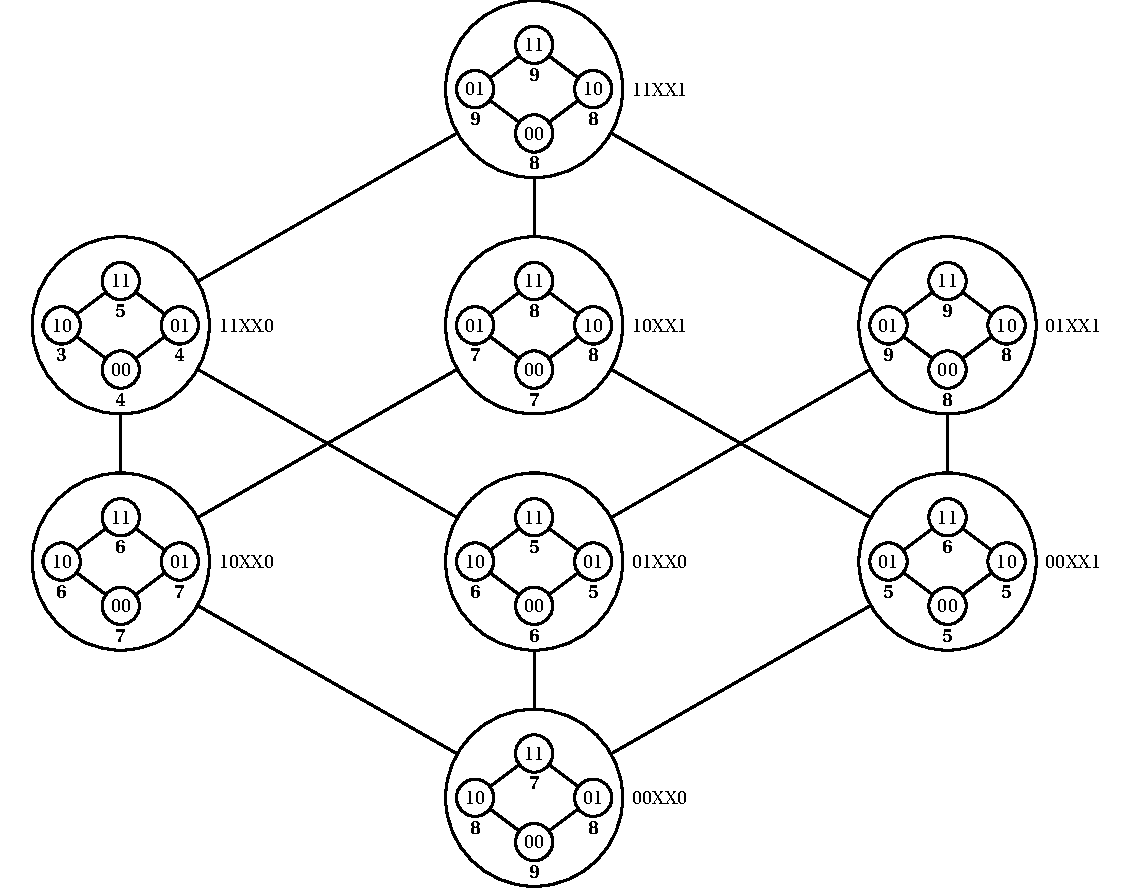
\includegraphics[clip=true, width=0.48\textwidth]{pucs/sample_run/A.pdf}
    }
    \end{tabular}   
    \end{center}
    \caption{Uma instância do problema U-Curve e o seu particionamento
    quando o conjunto de variáveis fixas $S'$ é composto pela primeira, 
    segunda e última variável. No reticulado externo, denotamos por $X$ 
    \foreignword{don't cares}, que são as variáveis livres do 
    particionamento. O subconjunto colorido em verde é o elemento de
    custo mínimo desta instância.}
    \label{fig:pucs:example:part_1}
\end{figure}

\begin{itemize}
    \item{Figura ~\ref{fig:pucs:example:lattice}: uma instância do 
        problema U-Curve com cinco características e com a função de 
        custo anotada ao lado dos nós do reticulado.} 
    \item{Figura ~\ref{fig:pucs:example:A}: o particionamento do espaço
        de busca quando são fixadas a primeira, segunda e última 
        característica.}
\end{itemize}

\begin{figure}[!ht]
    \begin{center}
    \begin{tabular}{l r}
    \centering
    \subfigure[] {
        \label{fig:pucs:example:B}
        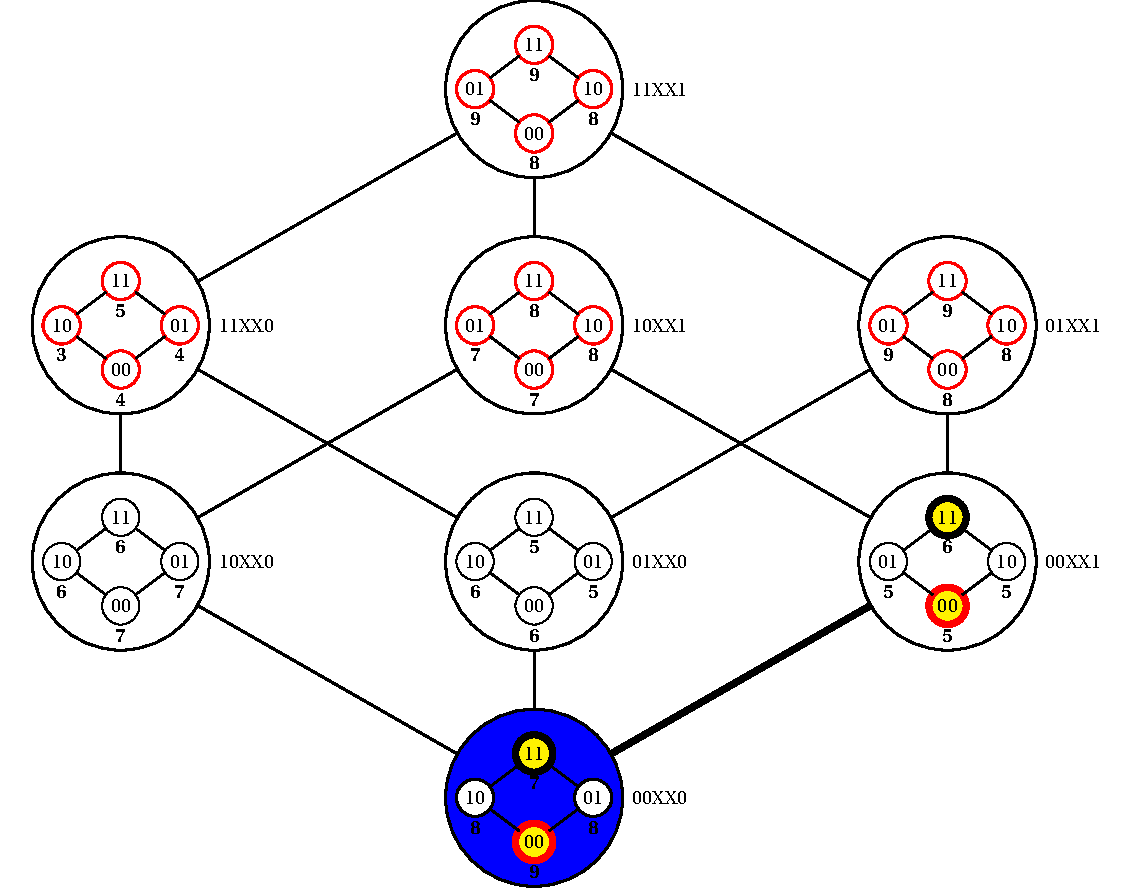
\includegraphics[ clip=true, width=0.48\textwidth]{pucs/sample_run/B.pdf}
    }
    &
    \subfigure[] {
        \label{fig:pucs:example:C}
        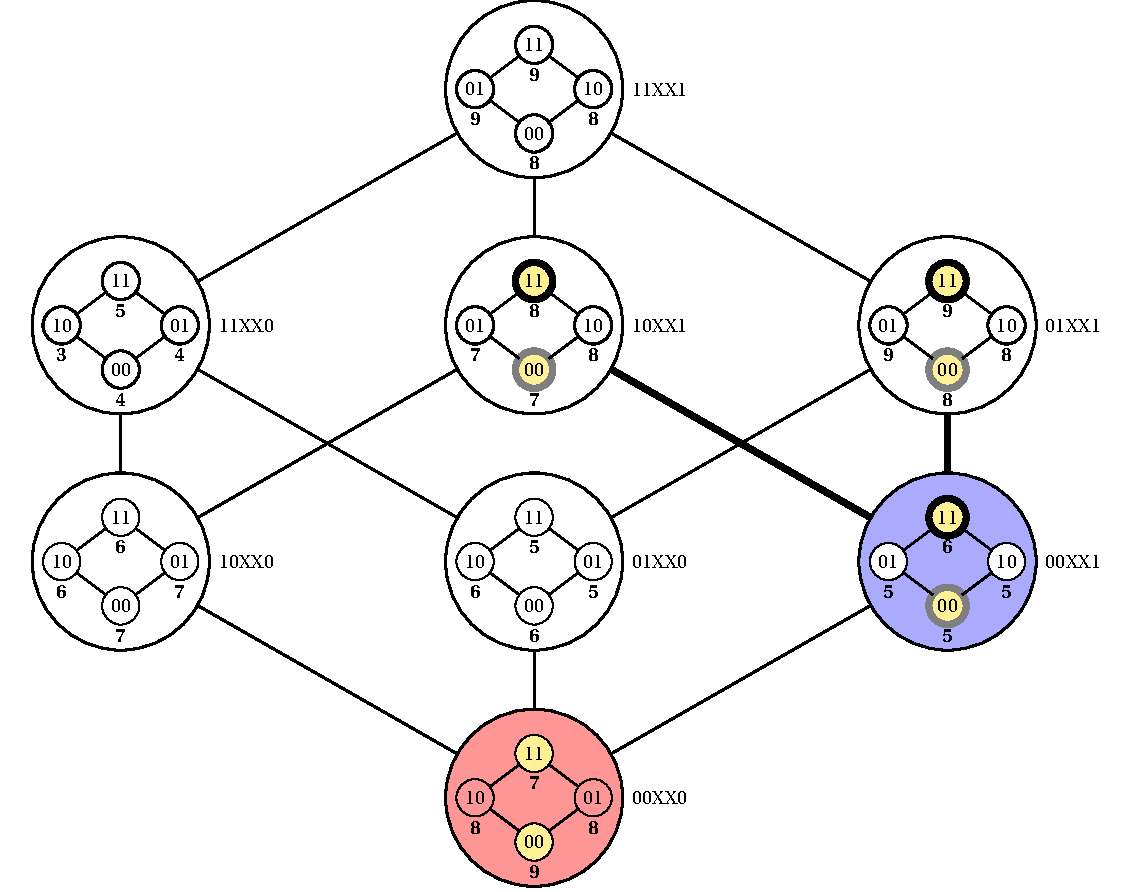
\includegraphics[clip=true, width=0.48\textwidth]{pucs/sample_run/C.pdf}
    }
    \\
    \subfigure[] {
        \label{fig:pucs:example:D}
        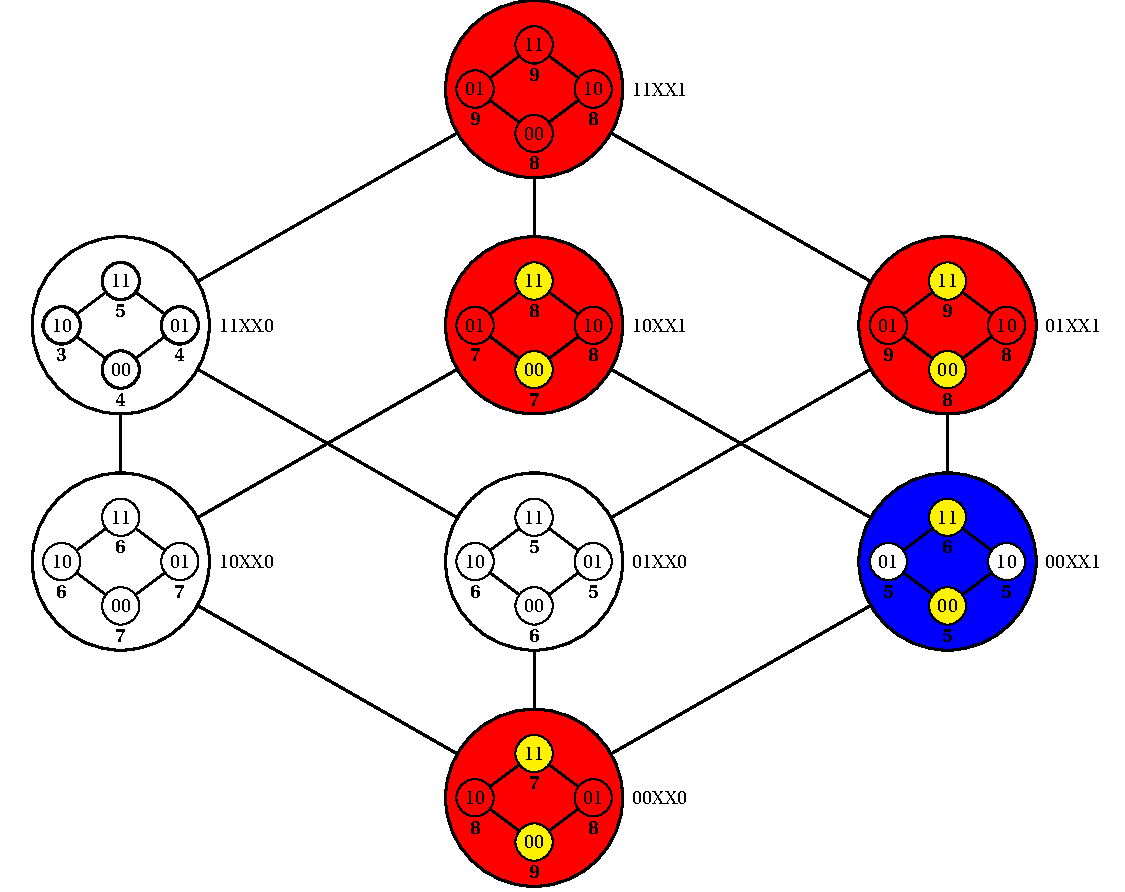
\includegraphics[ clip=true, width=0.48\textwidth]{pucs/sample_run/D.pdf}
    }
    &
    \subfigure[] {
        \label{fig:pucs:example:E}
        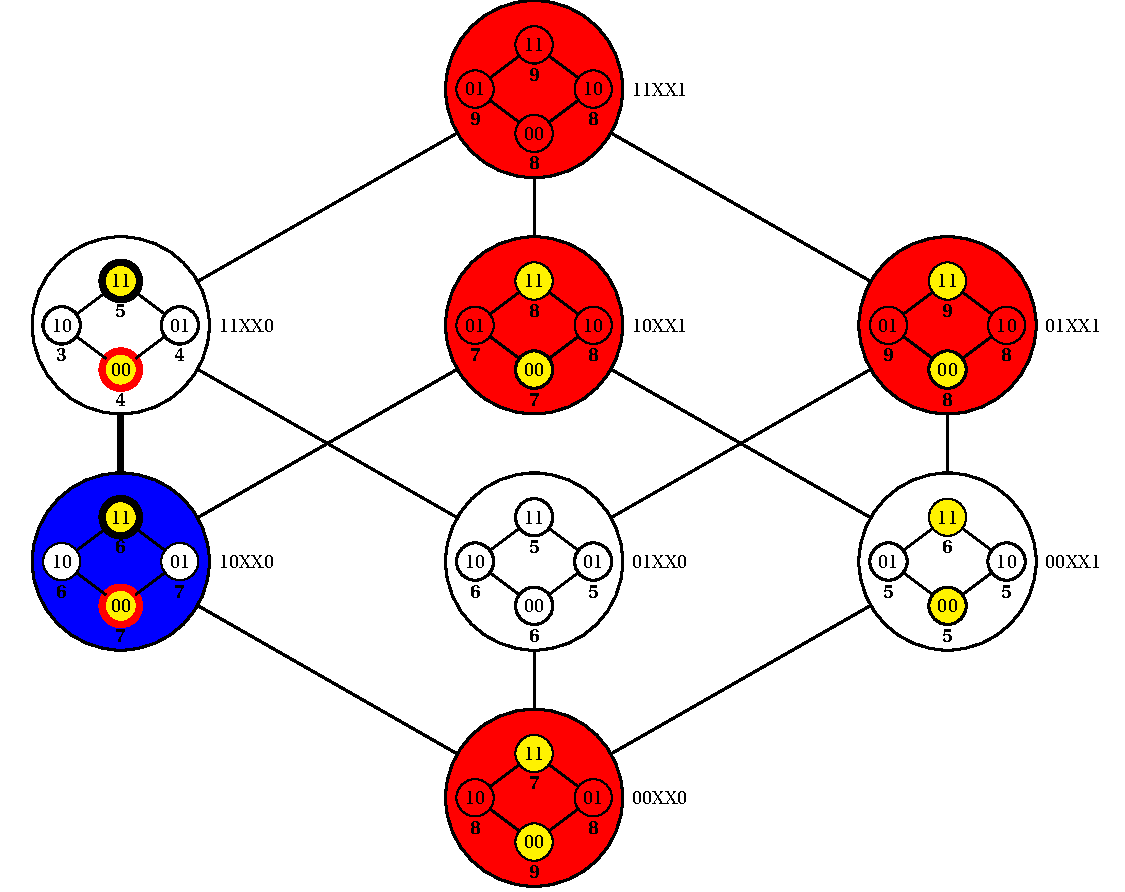
\includegraphics[clip=true, width=0.48\textwidth]{pucs/sample_run/E.pdf}
    }
    \end{tabular}   
    \caption{Dinâmica do algoritmo \algname{PUCS} ao resolver a instância apresentada na figura ~\ref{fig:pucs:example:part_1}}
    \label{fig:pucs:example:part_2}
    \end{center}
\end{figure}

\begin{itemize}
    \item{Figura ~\ref{fig:pucs:example:B} a parte 00XX0 é escolhida
        arbitrariamente para ser o início do passeio aleatório. O 
        vizinho 00XX1 é escolhido aleatoriamente como candidato a ser o
        próximo nó do passeio. Como o custo da ponta superior de 00XX1 
        (6) é menor do que o custo da ponta superior de 00XX0 (7), o
        intervalo de partes $[000, 000]$ é removido do espaço de busca.}
    \item{Figura ~\ref{fig:pucs:example:C} a pontas inferiores das 
        partes 10XX1 (7) e 01XX1 (8) têm custo maior do que a ponta 
        inferior de 00XX1 (5), portanto os intervalos de partes 
        $[101, 111]$ e $[011, 111]$ são removidos do espaço de busca.}
    \item{Figura ~\ref{fig:pucs:example:D} todos os vizinhos de 00XX1
        foram podados, portanto esta parte torna-se candidata a conter 
        o mínimo, e iniciamos um novo passeio.}
    \item{Figura ~\ref{fig:pucs:example:E} a parte 10XX0 é escolhida 
        arbitrariamente como início de passeio. O custo da ponta 
        superior de 10XX0 (6) é maior do que o custo da ponta superior
        de 11XX0 (5), portanto o intervalo de partes $[000, 100]$ é 
        removido do espaço de busca.} 
\end{itemize}

    
\begin{figure}[!ht]
    \begin{center}
    \begin{tabular}{l r}
    \centering
    \subfigure[] {
        \label{fig:pucs:example:F}
        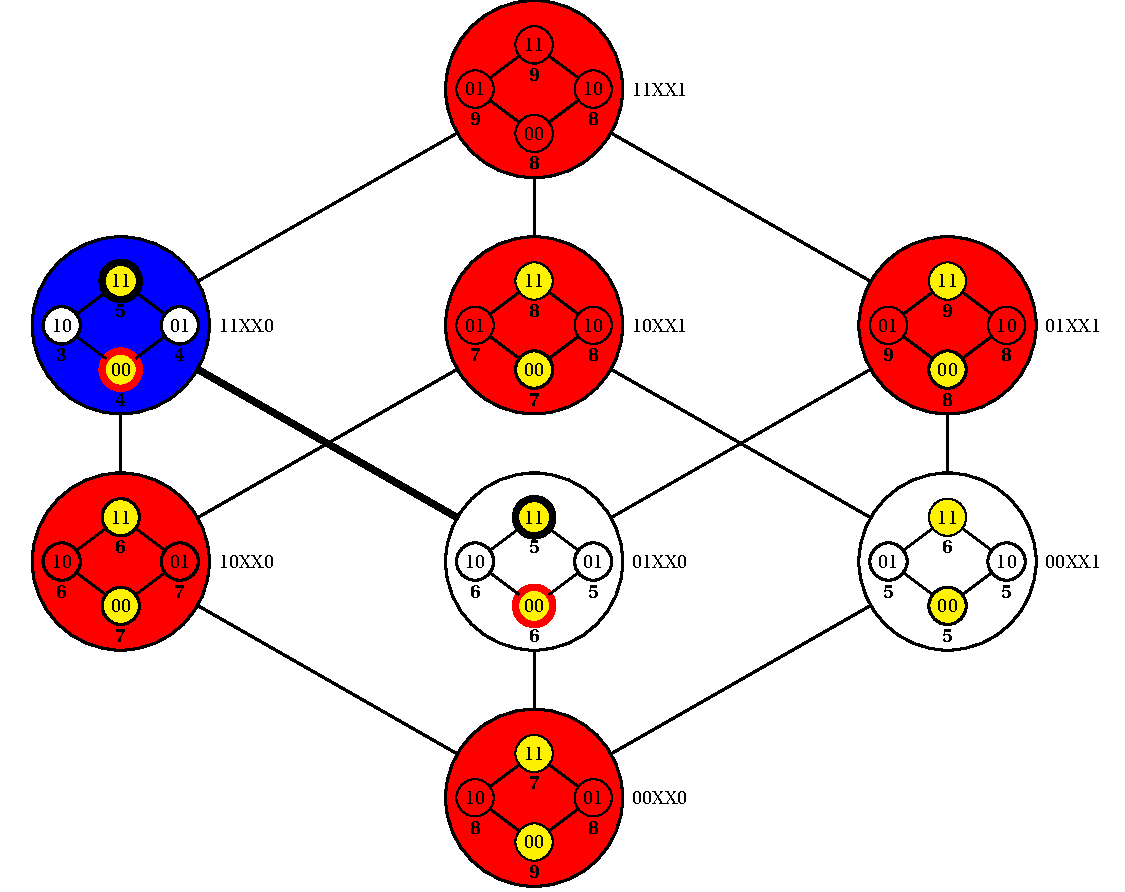
\includegraphics[ clip=true, width=0.48\textwidth]{pucs/sample_run/F.pdf}
    }
    &
    \subfigure[] {
        \label{fig:pucs:example:G}
        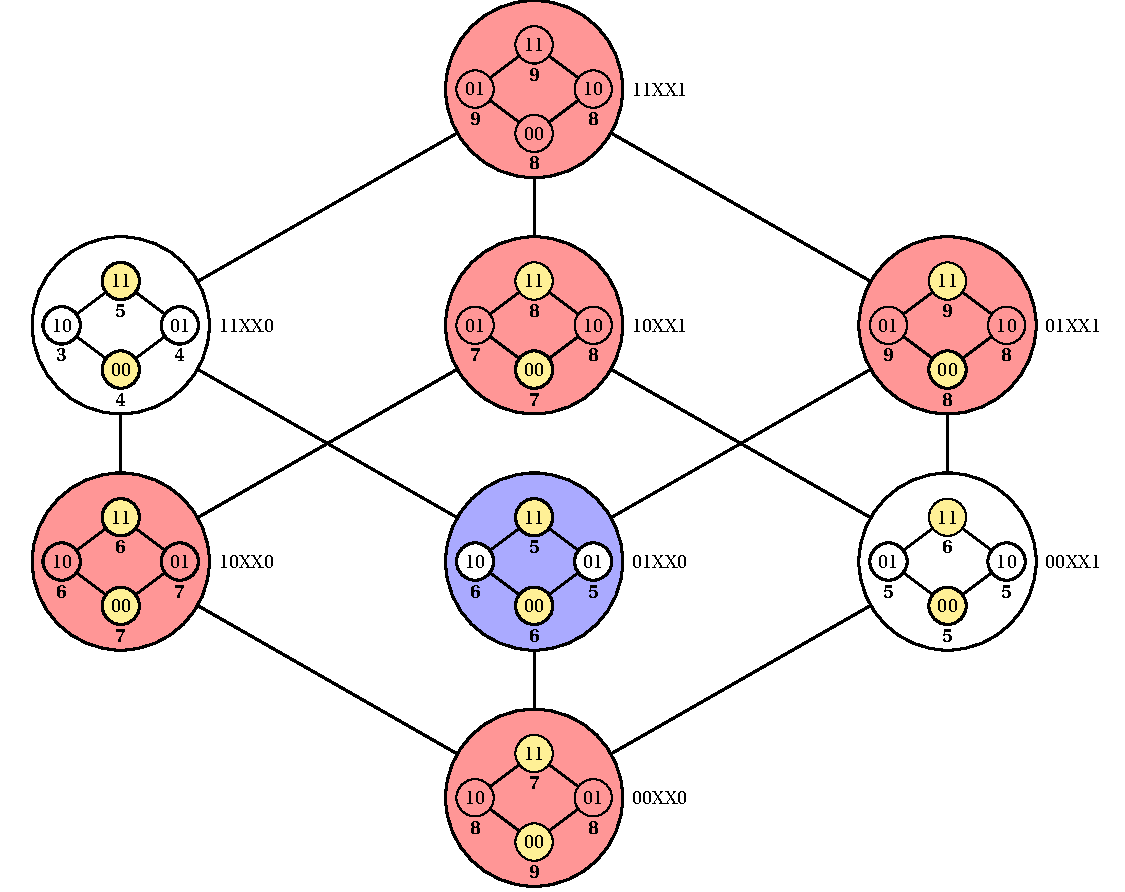
\includegraphics[clip=true, width=0.48\textwidth]{pucs/sample_run/G.pdf}
    }
    \\
    \subfigure[] {
        \label{fig:pucs:example:H}
        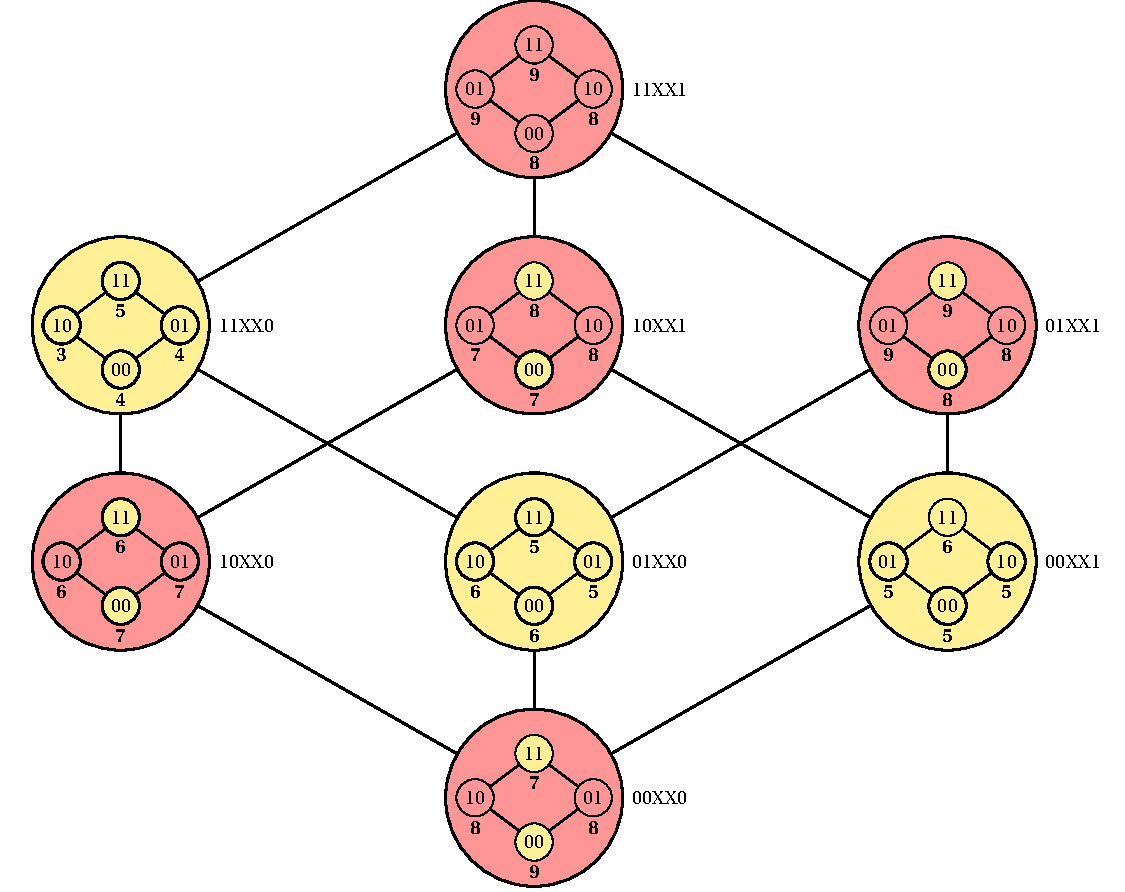
\includegraphics[ clip=true, width=0.48\textwidth]{pucs/sample_run/H.pdf}
    }
    &
    \subfigure[] {
        \label{fig:pucs:example:I}
        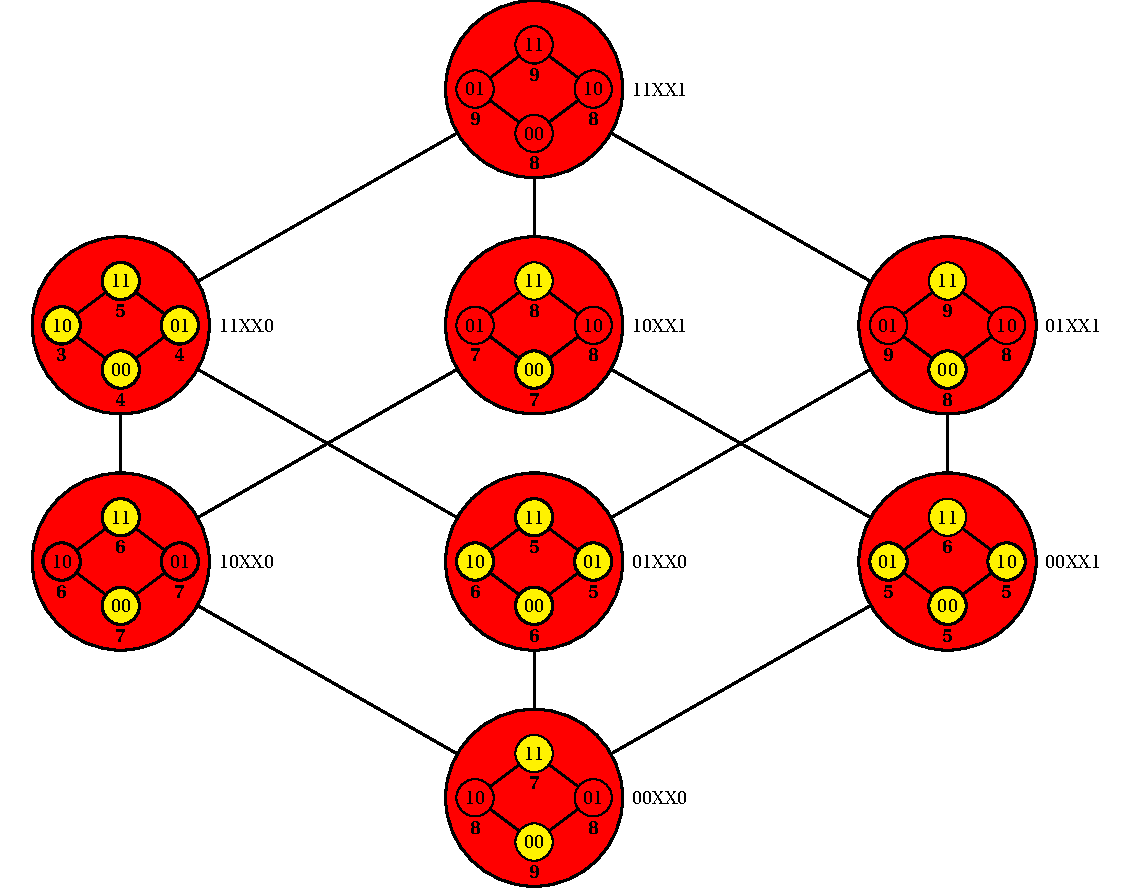
\includegraphics[clip=true, width=0.48\textwidth]{pucs/sample_run/I.pdf}
    }
    \end{tabular}   
    \caption{Continuação da figura ~\ref{fig:pucs:example:part_2}}%
    \label{fig:pucs:example:part_3}
    \end{center}
\end{figure}

\begin{itemize}
    \item{Figura ~\ref{fig:pucs:example:F} Nenhuma poda é realizada ao
        comparar 11XX0 com 01XX0, portanto a última torna-se o nó 
        corrente e a primeira torna-se candidata a conter o mínimo.} 
    \item{Figura ~\ref{fig:pucs:example:G} A parte 01XX0 torna-se o nó 
        corrente, mas como não possui vizinho no espaço de busca é 
        removida do espaço de busca e torna-se candidata a conter o 
        mínimo.}  
    \item{Figura ~\ref{fig:pucs:example:H} Todo nó foi removido do 
        espaço de busca por podas ou por visitas. Resolve-se as partes 
        candidatas a conter o mínimo.} 
    \item{Figura ~\ref{fig:pucs:example:I} O elemento de custo mínimo
        entre as partes é 11100, que é de fato a solução ótima do 
        problema com custo 3.} 
\end{itemize}


\subsection{Solução das partes} \label{sec:dynamics:solution}
Ao fim do passeio aleatório, teremos uma coleção de partes 
que precisam ser resolvidas para se obter o conjunto de custo mínimo. 
Nesta etapa, o \algname{PUCS} constrói para cada parte uma instância 
auxiliar do problema U-Curve que é equivalente ao problema original, 
porém restrito a parte de interesse. Seja $\langle S, c \rangle$ a 
instância do problema original e $S'$ o conjunto de variáveis fixas no 
particionamento feito pelo \algname{PUCS} neste problema, então,
dada uma parte $A \in \powerset(S')$, o conjunto de custo mínimo nesta 
parte é exatamente a solução ótima do problema U-Curve auxiliar 
$\langle \overline{S'}, c_A \rangle$ em que $c_A (X) = c (X \cup A)$ 
para qualquer $X \in \powerset(\overline{S'})$.

Para solucionar os problemas auxiliares, podemos chamar um outro 
algoritmo de seleção de características, ótimo ou sub-ótimo, e podemos 
inclusive chamar o próprio \algname{PUCS}, tornando o algoritmo 
recursivo. Chamamos o último algoritmo na sequência de chamadas 
recursivas de {\bf algoritmo base}; o \algname{PUCS} é algoritmo base 
apenas no caso em que cada parte contém apenas um elemento. A escolha do
algoritmo base é crítica no desempenho da chamada do \algname{PUCS} 
no que diz respeito a uso de recursos computacionais e também na 
qualidade da solução obtida.


\section{Parâmetros de funcionamento}
Na seção anterior apresentamos a dinâmica básica do algoritmo 
\algname{PUCS}, mas ainda não detalhamos como alguns passos acontecem. 
Estes passos dependem da escolha de alguns parâmetros do algoritmo: $p$,
$l$ e algoritmo base. Estes parâmetros são críticos para definir o 
desempenho e qualidade de resposta obtida pelo \algname{PUCS}.

O parâmetro $p$ define a quantidade de variáveis fixas no 
particionamento do espaço de busca e deve estar contido no intervalo 
$(0, 1]$, sendo a proporção de variáveis que devem ser fixadas; desta 
forma:
\begin{align*}
    |S'| & =  \ceil{|S| * p} \\
    |\overline{S'}| & = |S| - \ceil{|S| * p} \\
\end{align*}
Portanto, quanto maior o $p$ maior o tamanho do reticulado externo 
($|\powerset (S')|$) e menor o tamanho dos reticulados internos 
($|\powerset(\overline{S'})|$) e vice-versa. Isto significa que quando 
$p$ é pequeno, o \algname{PUCS} passa pouco tempo percorrendo o 
reticulado externo e a maior parte do tempo deve ser gasta na solução 
dos reticulados internos, pelo algoritmo base; quando $p$ é grande, o 
inverso deve acontecer.

Como vimos na seção ~\ref{sec:dynamics:solution}, a estrutura criada no
particionamento do problema nos permite fazer chamadas recursivas do 
\algname{PUCS}. O parâmetro $l$ determina a quantidade de chamadas 
recursivas acontecerão até que o algoritmo base seja chamado. Ao fazer 
chamadas recursivas estamos particionando o espaço de busca seguidas 
vezes e portanto, assim como o parâmetro $p$, quando aumentamos o valor
de $l$, o tamanho da parte que será resolvida pelo algoritmo base 
diminui. 
% É preciso notar que a quantidade total de partes cresce 
% rapidamente com o crescimento de $l$, O número total de partes após $l$
%chamadas recursivas do \algname{PUCS} é:
%\begin{align*}
    %\prod_{i = 1}^l 2^{n (1 - p)^{i - 1}p}
%\end{align*}


O algoritmo base determina como as partes serão resolvidas. Note que os 
teoremas ~\ref{theorem:pucs:pruning} e ~\ref{theorem:pucs:pruning_dual}
garantem que se a hipótese U-Curve for verdadeira, então todas as partes
que foram podadas do espaço de busca não contém o mínimo global, 
portanto se o algoritmo base é ótimo, então o \algname{PUCS} também é
ótimo. Se o algoritmo base for uma heurística, então o \algname{PUCS}
também se comporta como uma heurística, entretanto é provável que a 
solução encontrada pelo \algname{PUCS} seja melhor do que a solução 
dada pelo algoritmo base.
